%%%%%%%%%%%%%%%%%%%%%%%%%%%%%%%%%%%%%%%%%%%%%%%%%%%%%%%%%%%%%%%%%%%%%%%%%%%%%%%

\documentclass[12pt,twocolumn,tighten]{aastex62}
\usepackage{amsmath,amstext,amssymb}
\usepackage[T1]{fontenc}
\usepackage{apjfonts}
\usepackage[figure,figure*]{hypcap}
\usepackage{graphics,graphicx}
\usepackage{hyperref}
\usepackage{natbib}

\renewcommand*{\sectionautorefname}{Section} %for \autoref
\renewcommand*{\subsectionautorefname}{Section} %for \autoref

%% Reintroduced the \received and \accepted commands from AASTeX v5.2.
%% Add "Submitted to " argument.
\received{\today}
\revised{---}
\accepted{---}
\submitjournal{AAS journals.}
\shorttitle{WASP-4 is accelerating towards the Earth}

\begin{document}

\defcitealias{bouma_wasp4b_2019}{B19}

\title{WASP-4 is Accelerating Towards the Earth}
% ", Explaining its Decreasing Orbital Period"
% ": A Cautionary Tale in the Search for Tidal Orbital Decay"
% "An Explanation for WASP-4's Decreasing Orbital Period".
% "WASP-4's Decreasing Orbital Period: Solved."

\correspondingauthor{L. G. Bouma}
\email{luke@astro.princeton.edu}

%
% key authors:
%
\author[0000-0002-0514-5538]{L. G. Bouma}
\affiliation{ Department of Astrophysical Sciences, Princeton
University, 4 Ivy Lane, Princeton, NJ 08540, USA}
%
\author[0000-0002-4265-047X]{J. N. Winn}
\affiliation{ Department of Astrophysical Sciences, Princeton
University, 4 Ivy Lane, Princeton, NJ 08540, USA}

%
% contributing authors: alphabetical
%
\author[0000-0001-8638-0320]{A. W. Howard}
\affiliation{Cahill Center for Astrophysics, California Institute of
Technology, Pasadena, CA 91125, USA}
%
\author{S. B. Howell}
\affiliation{NASA Ames Research Center, Moffett Field, CA 94035, USA}
%
\author[0000-0002-0531-1073]{H. Isaacson}
\affiliation{Astronomy Department, University of California, Berkeley,
CA 94720, USA}
%
\author{H. Knutson}
\affiliation{Division of Geological and Planetary Sciences, California
Institute of Technology, Pasadena, CA 91125, USA}
%
\author{R. A. Matson}
\affiliation{NASA Ames Research Center, Moffett Field, CA 94035, USA}
%

\begin{abstract}
  Space and ground-based transit measurements of the hot Jupiter
  WASP-4b have recently shown that its orbital period appears to be
  decreasing.  Proposed explanations for the period change include
  tidal orbital decay, orbital precession, and light-travel time
  effects.  We present new radial velocity measurements of WASP-4,
  acquired with Keck-HIRES.  The data show that the system is
  accelerating towards the Earth at $\dot{\gamma} =
  -0.0422^{+0.0028}_{-0.0027}\,{\rm m}\,{\rm s}^{-1}\,{\rm day}^{-1}$.
  The implied period decrease explains most or all of WASP-4's
  changing orbital period as a light-travel time effect ($-5.94 \pm
  0.39~{\rm msec}\,{\rm yr}^{-1}$ implied, compared to $-8.64 \pm
  1.26~{\rm msec}\,{\rm yr}^{-1}$ observed).  Combining the radial
  velocities with new upper limits from speckle imaging, we find that
  the system's acceleration is likely caused by a 10-200$\,M_{\rm
  Jup}$ companion with semi-major axis between 10-100$\,$AU.  The
  statistics from \citet{knutson_friends_2014} imply that about 1 in 6
  hot Jupiters are expected to show comparable period decreases to
  WASP-4, due to acceleration by outer companions.  These
  period decreases will be increasingly measureable in coming years,
  because the precision of the period derivative measurement scales with
  the observing baseline to the power of 5/2.  Continued radial velocity monitoring
  of hot Jupiters is therefore essential to distinguish tidal orbital
  decay from line-of-sight accelerations.
\end{abstract}

\keywords{Exoplanet tides (497), Exoplanet dynamics (490), Radial velocity 
(1332), Transit timing variation method (1710)}

%%%%%%%%%%%%%%%%%%%%%%%%%%%%%%%%%%%%%%%%%%%%%%%%%%%%%%%%%%%%%%%%%%%%%%%%%%%%%%%

\section{Introduction}

The orbits of most hot Jupiters are unstable to tidal decay
\citep{counselman_outcomes_1973,hut_stability_1980,rasio_tidal_1996,levrard_falling_2009,matsumura_tidal_2010}.
The relevant issue is whether the timescale for tidal orbital decay is
shorter or longer than the timescale for main-sequence stellar
evolution.  This question depends on the uncertain rate at which
friction inside the star can damp the energy of tidal oscillations and
thereby shrink the orbit (as reviewed by \citealt{Mazeh2008} and
\citealt{ogilvie_tidal_2014}).

Indirect studies of age and angular momentum indicators including the
hot Jupiter semi-major axis distribution, host star spin rates, and
galactic velocity dispersions have led to estimates for the inspiral
timescale that vary from much less to much greater than the
main-sequence evolution time  ({\it e.g.},
\citealt{jackson_observational_2009}, \citealt{teitler_why_2014},
\citealt{penev_empirical_2018}, \citealt{cameron_hierarchical_2018},
\citealt{hamer_schlaufman_2019}).  Direct measurements of tidal
orbital decay through transit and occultation timing could provide an
empirical resolution.  For instance, combined transit timing and
radial velocity measurements for WASP-12b have shown that its secular
period decrease of $\approx$30 milliseconds per year is probably due
to tidal orbital decay
\citep{maciejewski_departure_2016,patra_2017,yee_orbit_2020}.

This study highlights a point that, though obvious, has perhaps not
yet received due attention.  The point is that observational programs
aimed at identifying orbital decay in hot Jupiters through transit
timing will be crippled without concurrent long-term radial velocity
monitoring.  The reason is that line-of-sight accelerations due to
outer companions \citep[{\it e.g.},][]{agol_detecting_2005} and tidal
orbital decay both initially manifest identically in transit times, as
a non-zero period derivative.  Massive outer companions to hot
Jupiters are the norm; \citet{bryan_statistics_2016} calculated an
occurrence rate of $60.9^{+5.2}_{-5.6}\%$ for outer companions to hot
Jupiters with masses from 1-20$\,$$M_{\rm Jup}$ and semi-major axes
from 5-100$\,$AU.  Therefore it could very well be that more hot
Jupiters will show shrinking orbital periods due to long term
accelerations than due to tidal orbital decay.

The main focus of this study is the hot Jupiter WASP-4b, which has an
orbital period that appears to be decreasing by about 10 milliseconds
per year.  We discovered the timing variations by combining data from
TESS \citep{ricker_transiting_2015} with a decade of ground-based
observations \citep[][hereafter
\citetalias{bouma_wasp4b_2019}]{bouma_wasp4b_2019}.  Thereafter,
\citet{southworth_transit_2019} reported 22 new transit times for the
system, and found an updated decay rate of $\dot{P} = -9.2 \pm 1.1$
milliseconds per year. The \citeauthor{southworth_transit_2019} decay
rate was $\approx$3$\sigma$ less rapid than that found by
\citetalias{bouma_wasp4b_2019}, but the conclusions of the studies
were otherwise similar.  A separate study by \citet{baluev_2019}
reported additional archival transit light curves of WASP-4b from
TRAPPIST and select other observers.  \citet{baluev_2019} pointed out
that when using lower-precision subsets of the available transit data,
the case for a decreasing period worsened.

To determine the origin of the period change, we acquired four
additional radial velocity measurements using Keck-HIRES, extending
the RV baseline from 3 to 9 years.  Previously, the five available
HIRES radial velocities suggested a weak ($\approx$$2\sigma$) linear
trend \citep{knutson_friends_2014}.  Our new measurements reveal a
line-of-sight acceleration of $\dot{\gamma} =
-0.0422^{+0.0028}_{-0.0027}\ {\rm m\,s^{-1}\,day^{-1}}$.  This
translates to an expected period decrease from the light-travel time
effect of -5.9 milliseconds per year---about commensurate with what is
observed from transits.  While the apparent period change caused by a
line-of-sight acceleration has been referred to as the ``R{\o}mer
effect'' \citep{yee_orbit_2020}, we prefer to avoid this term, which
typically signifies arrival time delay due to observatory motion. We
are discussing the Doppler effect seen by a stationary observer for a
source with constant line-of-sight acceleration.

In the following, Section~\ref{sec:observations} collects the
available transit data and presents the new radial velocity and
speckle imaging observations.  Section~\ref{sec:analysis} analyzes the
data, and finds that they yield a picture in which the WASP-4 system
is accelerating towards our line-of-sight, likely due to the pull of a
brown or M-dwarf companion.  Section~\ref{sec:discussion} places this
result in the broader context of orbital decay searches, and points
out that line-of-sight accelerations, {\it i.e.}, ``false positive
orbital decay signals'', are relatively common in the hot Jupiter
population.  Section~\ref{sec:conclusions} offers concluding remarks.

\section{Observations}
\label{sec:observations}

\subsection{Transits}

Table~1 lists the transit times we collected for our analysis.  We
include data from the peer-reviewed literature for which {\it (i)} the
analysis was based on observations of a single transit, {\it (ii)} the
midpoint was fitted as a free parameter, and {\it (iii)} the time
system specified both the leap second correction (TDB or UTC) and also
whether any barycentric or heliocentric corrections had been
performed.

% FIXME : verify with Michael Gillon that this is true. (P. Evans
% done)
The majority of times are identical to those we collected in
\citetalias{bouma_wasp4b_2019}.  Twenty-two new times reported by
\citet{southworth_transit_2019} are included.  These transits were
observed from the 3.58m NTT and Danish 1.54m telescopes at La Silla,
and the SAAO 1.0m telescope.
% Five of the twenty-two occurred at simultaneous epochs as transits
% previously reported by \citet{hoyer_tramos_2013}.

Additional timing measurements were also recently made available by
\citet{baluev_2019}, based on a homogeneous analysis of archival
ground-based observations.
We included twelve of their ``high quality'' transit times from
TRAPPIST (six transits), El~Sauce (four transits), and
\citet{petrucci_no_2013}.  For TRAPPIST and El~Sauce, we verified with
the original observers that correct barycentric and leap-second
corrections had been performed (M.~Gillon, P.~Evans, priv{.} comm{.}).
We omitted the fourteen remaining \citeauthor{baluev_2019}
ETD\footnote{\url{http://var2.astro.cz/ETD}} times due to ambiguity in
whether leap-second corrections had or had not been performed.

The four available occultations tabulated by
\citetalias{bouma_wasp4b_2019} have neglegible statistical value due
to their large uncertainties, and we forgo their use in this analysis.

\subsection{Radial velocities}

After identifying the period decrease in
\citetalias{bouma_wasp4b_2019}, we acquired four additional radial
velocity measurements with the Keck High Resolution Echelle
Spectrometer (HIRES; \citealt{vogt_hires_1994}).  Our observations
were acquired using the standard setup and reduction techniques of the
California Planet Survey \citep{howard_cps_2010}.  Previously, the
HIRES data-points spanned 2010 to 2013 \citep{knutson_friends_2014}.
Our new measurements triple the HIRES observing baseline to nine
years.

The complete set of radial velocity observations is given in Table~2.
Along with the 2010-2019 HIRES observations, there are also
measurements from CORALIE and HARPS.  Following
\citetalias{bouma_wasp4b_2019}, we included the CORALIE measurements
from \citet{wilson_wasp-4b_2008} and \citet{triaud_spin-orbit_2010},
using the homogeneous values calculated by the latter authors.

For HARPS, we included the values reported by
\citet{pont_determining_2011} and \citet{husnoo_observational_2012}.
While \citet{triaud_spin-orbit_2010} also acquired HARPS data over
three nights for Rossiter-McLaughlin observations, these data were
reduced with a non-standard pipeline, and so are systematically offset
from the remaining HARPS data.  In our final fit, we therefore omitted
the three \citet{triaud_spin-orbit_2010} nights.  We did nonetheless
experiment with using the recent \citet{trifonov_public_2020}
re-reductions, which allowed us to include two calibration RVs taken
as part of the \citet{triaud_spin-orbit_2010} program. The decision
regarding whether to include or omit these points did not
noticeably affect our results.


\subsection{Speckle imaging}

An initial analysis of the new HIRES observations led to our detection
of a linear trend in the residuals after fitting out the orbit of
WASP-4b.  This prompted us to acquire speckle images using Zorro at
Gemini-South \citep[see][and the instrument
web-pages\footnote{\url{www.gemini.edu/sciops/instruments/alopeke-zorro/}}]{scott_nessi_2018}.
Zorro is a dual-channel speckle interferometer employing narrow-band
filters centered at 562$\,$nm and 832$\,$nm.  

We observed WASP-4 twice, on the night of September 11-12 with
relatively poor seeing (1.2$''$) and also on the night of September
28-29.  Over each observation, we acquired three sets of 1000
60$\,$msec exposures.  If a companion is present, the autocorrelation
functions of these speckle images reveal a characteristic interference
pattern. This pattern in then used to determine the properties of the
detected companion and to produce a reconstructed image.  Using the
reconstructed speckle images,  contrast curves are produced yielding
5-sigma detection limits  (see \citealt{howell_speckle_2011}).  No
companions were detected, and the second night, which had better
seeing (0.6$''$), also produced the more constraining result.  The
832$\,$nm limits were the most useful to us given that faint
companions are redder than the host star.  We therefore opted to use
the 832$\,$nm September 28-29 contrast limits for the remaining
analysis.


\section{Analysis}
\label{sec:analysis}

\subsection{Transits}
\label{sec:transit_analysis}

\begin{figure}[t]
	\begin{center}
		\leavevmode
		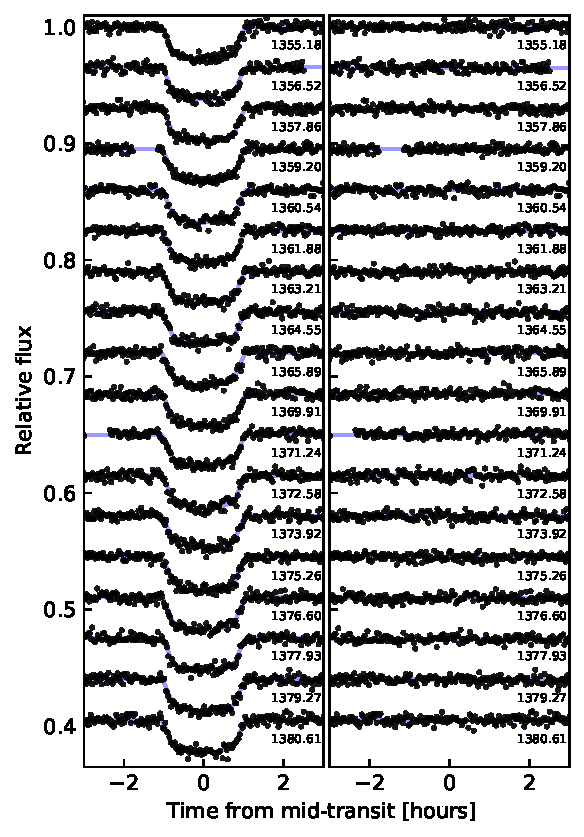
\includegraphics[width=0.47\textwidth]{f1.pdf}
	\end{center}
	\vspace{-0.7cm}
  \caption{ {\bf Timing residuals and best-fit models for WASP-4b.}
  The vertical axis shows the observed transit times minus the
  calculated times assuming a constant orbital period.  More opaque
  points correspond to more precise data.  The $\pm1\sigma$
  uncertainties of the quadratic ephemeris 
  are shown in blue.
  The binned TESS point (yellow star) is the weighted average of 18
  TESS transits and is binned for display purposes only.  The models
  were fitted to all of the individual transit times.
  \label{fig:times}
	}
\end{figure}

We considered two models for the observed transit times.  The first
model assumes a constant orbital period $P$ on a circular orbit:
\begin{align}
  t_{\rm tra}(E) &= t_0 + PE,
\end{align}
where $E$ is the integer transit number and $t_0$ is a reference
epoch.  The second model assumes that the period changes at a steady
rate:
\begin{align}
  t_{\rm tra}(E) &=
    t_0 + PE +
    \frac{1}{2} \frac{{\rm d}P}{{\rm d}E} E^2.
  \label{eq:quadratic_model}
\end{align}
The free parameters are the reference epoch $t_0$, the period at the
reference epoch $P$, and the period derivative, ${\rm d}P/{\rm d}t =
(1/P) {\rm d}P/{\rm d}E$.  We defined the epoch numbers such that
$E=0$ is near the weighted average of the observed times.  This helps
to reduce the covariance between $t_0$ and $P$.  A third possible
model that we did not consider for reasons that will become apparent
is a precessing, eccentric orbit \citep[{\it
e.g.},][]{gimenez_revision_1995,patra_2017}.

We fitted each of the two models by assuming a Gaussian likelihood and
sampling over the posterior probability distributions.  We sampled the
posterior using the algorithm proposed by
\citet{goodman_ensemble_2010} and implemented by
\citet{foreman-mackey_emcee_2013} in \texttt{emcee}.  The prior for
the quadratic model allowed the period derivative to have any sign.

Figure~\ref{fig:times} shows the observed transit times, minus the
best-fit constant period model.  The best-fitting constant-period
model has 91 degrees of freedom, $\chi^2 = 276$,  and $\chi^2_{\rm
red}=3.0$.  The best-fitting quadratic model has 90 degrees of freedom,
$\chi^2 = 183$, and $\chi^2_{\rm red}=2.0$.  The difference in the
Bayesian information criteria (BIC) between the linear and quadratic
and models is $\Delta {\rm BIC} = 89$, strongly favoring the
quadratic model \citep{kass_bayes_1995}.

From the reduced $\chi^2$ values, we can surmise that neither model
entirely describes the transit data---there
must be some additional source of signal or noise. In
\citetalias{bouma_wasp4b_2019}, we found that the quadratic model for the
(sparser) transit data gave $\chi^2_{\rm red}=1.0$.  The worsened
$\chi^2_{\rm red}$ could reflect underestimated statistical
uncertainties in any of our transit measurements.  It could also
reflect systematic errors in the time-systems in which the transit
measurements were recorded, though we have taken every caution against
this latter possibility.

One approach to analyzing such data would be to inflate the transit
measurement uncertainties, and lower the reduced $\chi^2$.  We do not
think that such an approach is warranted, because it would not change
the result that the quadratic model is strongly preferred.  Instead,
we opt to simply inflate the uncertainties reported for each model by
a factor of $(\chi^2_{\rm red})^{1/2}$, or $\approx$1.73$\times$ for the
linear model, and $\approx$1.41$\times$ for the quadratic.

The resulting best-fit period derivative for the quadratic model is 
\begin{equation}
\dot{P}
  = - (2.74 \pm 0.28)\times 10^{-10}
  = - 8w.64 \pm 1.26~{\rm msec}\,{\rm yr}^{-1}.
  \label{eq:dP_dt_obs}
\end{equation}
This agrees to within $1\sigma$ of the value reported by
\citet{southworth_transit_2019} ($\dot{P} = - 9.2 \pm 1.1~{\rm
ms}\,{\rm yr}^{-1}$).  It is $\approx$2.3$\sigma$ larger than the rate
of period decrease we previously reported \citepalias[$- 12.6 \pm 1.2~{\rm
ms}\,{\rm yr}^{-1}$;][]{bouma_wasp4b_2019}, presumably because of the
new data from \citeauthor{southworth_transit_2019} and
\citeauthor{baluev_2019}  The other best-fit transit timing model
parameters are reported in Table~3.



\subsection{Radial Velocities: WASP-4's acceleration towards the Earth}

\begin{figure}[t]
	\begin{center}
		\leavevmode
		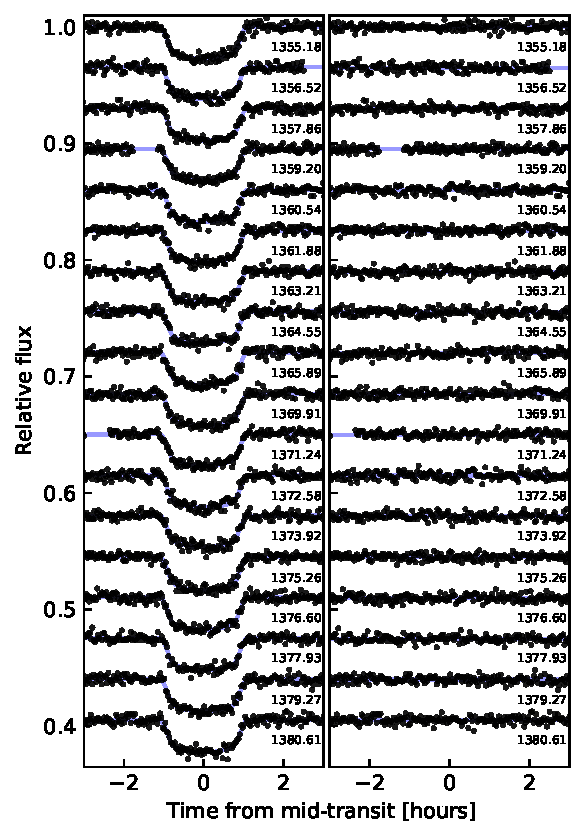
\includegraphics[width=0.47\textwidth]{f2.pdf}
	\end{center}
	\vspace{-0.7cm}
	\caption{
    {\bf Radial velocity residuals of WASP-4.} The best-fit
    Keplerian orbit of WASP-4b has been subtracted.  The linear trend
    inferred from the RV data is shown with a black line, with
    $1\sigma$ errors in gray.  The trend that would be needed to
    produce the period decrease seen in transits ($\dot{P}= - 8.64 \pm
    1.26~{\rm msec}\,{\rm yr}^{-1}$) is indicated in purple.  The four
    new RV measurements presented in this work increase the
    significance of the radial velocity trend from $\approx$2$\sigma$
    to 15$\sigma$.
	\label{fig:rvs}
  \vspace{-0.3cm}
	}
\end{figure}

Our initial model for the radial velocity data was a single Keplerian
orbit, plus instrument offsets, jitters, and a long-term linear trend
\citep[][\texttt{radvel}]{fulton_radvel_2018}.  We set Gaussian priors
on the orbital period and time of inferior conjunction using the
values from Table~4 of \citetalias{bouma_wasp4b_2019}, and fixed
WASP-4b's eccentricity to zero
\citep{beerer_secondary_2011,knutson_friends_2014,bonomo_gaps_2017}.
The free parameters were the velocity semi-amplitude, the instrument
zero-points, an additive ``white noise'' instrument jitter for each
instrument, and a linear ($\dot{v_{\rm r}}$) acceleration term.  We
also considered a model without the linear trend, and found that it
was disfavored by $\Delta {\rm BIC}=73$.

In the preferred ``planet+linear trend'' model, WASP-4 is accelerating
towards our line-of-sight at high confidence,
\begin{equation}
  \dot{v}_{\rm r} = \dot{\gamma} = 
     -0.0422^{+0.0028}_{-0.0027}
     \,{\rm m}\,{\rm s}^{-1}\,{\rm day}^{-1}.
\end{equation}
For comparison, before our new measurements, $\dot{\gamma}$ was
thought to be about five times smaller, and had marginal statistical
significance \citep{knutson_friends_2014,bouma_wasp4b_2019}.

The system's acceleration towards our line-of-sight causes a decrease
in the apparent orbital period:
\begin{align}
  \dot{P}_{\rm\,RV} &= \frac{\dot{v}_{\rm r} P}{c},
\end{align}
or in more convenient units,
\begin{align}
  \dot{P}_{\rm\,RV} &= 105{.}3\,{\rm msec}\,{\rm yr}^{-1} \
  \left( \frac{P}{{\rm day}} \right)
  \left( \frac{\dot{\gamma}}{ {\rm m}\,{\rm s}^{-1}\,{\rm day}^{-1}} \right).
\end{align}
For WASP-4, this yields
\begin{align}
  \dot{P}_{\rm\,RV} &= -5.94 \pm 0.39\,{\rm msec}\,{\rm yr}^{-1}.
\end{align}
The majority of the period decrease seen in transits ($\dot{P}= -
8.64 \pm 1.26~{\rm msec}\,{\rm yr}^{-1}$) therefore seems to be caused by the
acceleration of the host star.

An important consideration is whether the measured RV trend is
correlated with stellar activity.  We investigate this by analyzing
WASP-4's emission in the Ca II H \& K lines, as quantified with the
chromospheric $S$-index \citep{wright_chromospheric_2004}.  We only
examined the HIRES velocities for this step, since they are the main
source of signal for our analysis.  First, we subtracted the orbital
solution from the Keck-HIRES velocities.  Then, following
\citet{bryan_statistics_2016,bryan_excess_2019}, we calculated the
Spearman rank correlation coefficient between the $S$-index and the
orbit-subtracted velocities.  We found a correlation coefficient of
0.16. This correlation is not statistically significant; the
corresponding $p$-value is 0.65.  Furthermore, inspection of the
$S$-index timeseries did not show secular or sinusoidal trends, as
would be expected if we were observing a long-term magnetic activity
cycle.  The $S$-index values are included in Table~2.  We conclude
that it is highly unlikely that the linear trend is caused by stellar
activity.


\subsection{Constraints on companion masses and semi-major axes}

\begin{figure}[!t]
	\begin{center}
		\leavevmode
		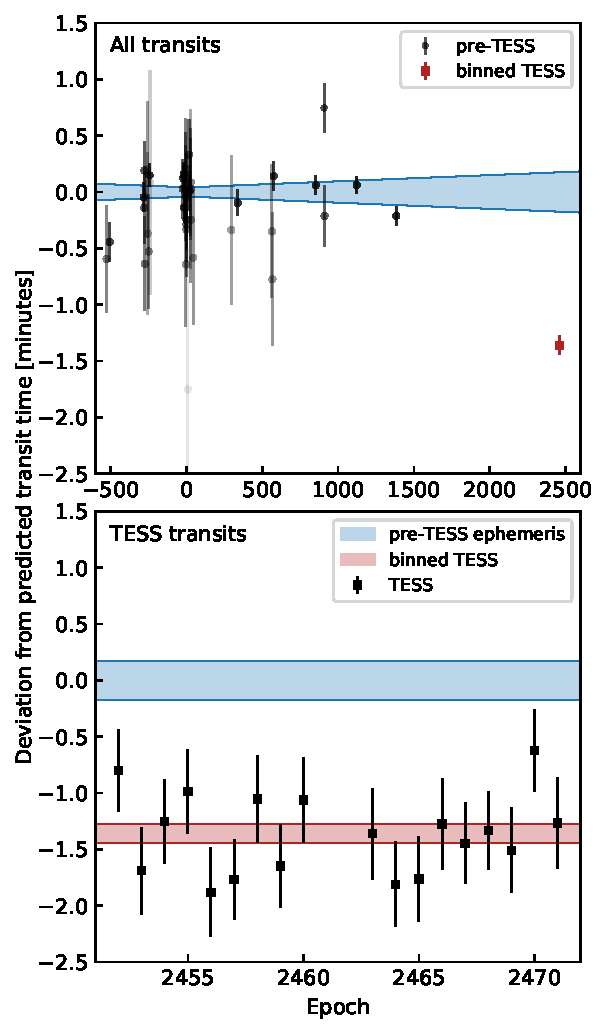
\includegraphics[width=0.47\textwidth]{f3.pdf}
	\end{center}
	\vspace{-0.7cm}
    \caption{
      {\bf Zorro contrast limits derived from point-source
      injection-recovery experiments.} Sources below the curve would
      have been detected.  The inset shows the speckle image
      reconstructed from 1000 60 millisecond frames in an 832$\,$nm
      bandpass, and acquired on September 28, 2019.  The image scale
      is $2.46''\times2.46''$.
    }
    \label{fig:zorro}
\end{figure}

\begin{figure*}[t]
	\begin{center}
		\leavevmode
		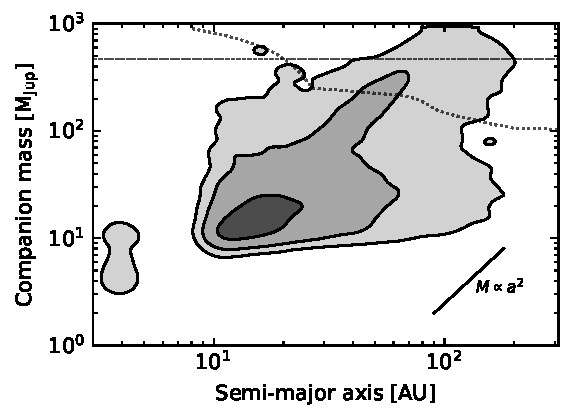
\includegraphics[width=0.73\textwidth]{f4.pdf}
	\end{center}
	\vspace{-0.6cm}
	\caption{
    {\bf Masses and semi-major axes of companions that meet
    requirements of both the radial velocities and the speckle
    imaging.} The likelihood inferred from radial velocities is shown
    in grayscale, and the region excluded from the speckle imaging is
    indicated.  The expected mass to semimajor-axis degeneracy is
    shown with a black line.
	\label{fig:mass_sma}
  \vspace{-0cm}
	}
\end{figure*}


Given a linear radial velocity trend, we can place lower-limits on the
mass and semi-major axis of additional bodies in the system.  For a
quick estimate of the minimum mass required to explain the linear
trend in WASP-4, we turn to \citet{feng_california_2015}.  As they
discuss, the scenario that yields the minimum companion mass for a
system with a linear trend is a companion with $e\approx0.5$ and
$\omega=90^\circ$.  Substituting $P\approx 1.25\tau$ and $K \approx
0.5\tau \dot{\gamma}$ into the mass function \citep[{\it
e.g.},][]{wright_efficient_2009} yields
\begin{equation}
 M_{\rm min} \approx 5.99\,M_{\rm Jup}
  \left( \frac{\tau}{{\rm yr}} \right)^{4/3}
  \left| \frac{\dot{\gamma}}{{\rm m\,s^{-1}\,day^{-1}}} \right|
  \left( \frac{M_\star}{{M_\odot}} \right)^{2/3},
\end{equation}
where $\tau$ is the observing baseline.  For WASP-4, this gives
$M_{\rm min} = 4.9 M_{\rm Jup}$.  Higher masses are allowed for
companions that orbit further from the star: at fixed $\dot{\gamma}$,
$M_{\rm comp} \propto a^2$
\citep{torres_substellar_1999,liu_crossing_2002}.

High-resolution images can further limit the available parameter space
by setting an upper limit on the semimajor axis, and a maximum
brightness (and thereby mass) of any putative companions.  The
procedure we use to combine constraints from both radial velocities
and high resolution imaging has been developed by
\citet{wright_linear_trends_2007}, \citet{crepp_trends_2012},
\citet{montet_trends_2014}, \citet{knutson_friends_2014},
\citet{bryan_statistics_2016,bryan_excess_2019}, and others.

\paragraph{Speckle imaging constraints}

First, we would like to convert the contrast ratios obtained through
the Zorro imaging (Figure~\ref{fig:zorro}) to limits on the masses of
putative companions and their separations from the host star.

To do this, we followed \citet{montet_trends_2014}, and opted to
employ the \citet{baraffe_evolutionary_2003} models for substellar
mass objects and the MIST isochrones for stellar mass objects
\citep{paxton_modules_2011,paxton_modules_2013,paxton_modules_2015,dotter_mesa_2016,choi_mesa_2016}.
We assumed that the system age was 5 Gyr, so that companions would
have fully contracted.

Due to the custom filters of the Zorro imager, and corresponding lack
of synthetic photometry, we further assumed that all sources had
blackbody spectra. While this is a simplification, we do not
readily have access to the planetary and stellar atmosphere models
needed for the consistent calculation with the \texttt{COND03} and
\texttt{MESA} models.  We therefore adopted the effective temperatures
and bolometric luminosities from the \citet{baraffe_evolutionary_2003}
and MIST isochrones.  Using these theoretical quantities and the
empirically-measured Zorro bandpasses, we calculated absolute
magnitudes in the 562 and 832 nm Zorro bands for stellar and planetary
mass companions.  Applying the same calculation to WASP-4 itself using
the effective temperature and bolometric luminosity from
\citetalias{bouma_wasp4b_2019}, we derived the transformation from
contrast ratio to companion mass.  The resulting limits are shown in
Figure~\ref{fig:mass_sma}.


\paragraph{Radial velocity constraints}

To derive constraints on possible companion masses and separations
from the radial velocities, we mostly followed the procedure of
\citet{bryan_excess_2019}. 

We began by defining a $128\times128$ grid in true planetary mass and
semimajor axis, with even logarithmic spacing from 1 to 900$\,$$M_{\rm
Jup}$ and 3 to 500$\,$${\rm AU}$.  We then considered the possibility
that an additional companion in any particular cell could explain the
observed linear trend.  In each cell, we simulated 512 hypothetical
companions.

We assigned each companion a mass and semimajor axis from log-uniform
distributions within the grid cell. We drew the inclination from a
uniform distribution in $\cos i$.  For companion masses less than
$10\,M_{\rm Jup}$, we drew the eccentricity from
\citet{kipping_beta_2013}'s long-period exoplanet Beta distribution
($a=1.12$, $b=3.09$).  If the companion mass exceeded $10\,M_{\rm
Jup}$, we drew the eccentricity from the power-law $p_e \propto
e^\eta$ reported by \citet{moe_mind_2017} in their Equation~17 ($\eta
\approx 0.5$ for most orbital periods).  The long-period exoplanet and
long-period binary eccentricity distributions are quite different: the
exoplanet distribution is ``bottom-heavy'', with eccentricities
preferentially close to zero.  The binary star distribution is
``top-heavy'', with eccentricities closer to one.  We chose a mass
cutoff of $10\,M_{\rm Jup}$ to separate the two regimes based on the
bound observed by \citet{schlaufman_evidence_2018} between giant
planets and brown dwarfs, though this value is also close to the
$13\,M_{\rm Jup}$ deuterium-burning limit \citep[{\it
e.g.},][]{burrows_nongray_1997}.

For each simulated companion, we then drew a sample from the converged
chains of our initial model of WASP-4b. We subtracted the planet's
orbital solution, leaving RV points with a linear trend.  Given
$(a_{\rm c}, M_{\rm c}, e_{\rm c})$ for each simulated outer
companion, and the fixed instrument offsets and jitters from the MCMC
chains, we then performed a maximum likelihood fit for the time and
argument of periastron of the outer simulated companion.  We converted
the resulting $128\times128\times512$ cube of log-likelihood values to
probabilities, and averaged over the samples in each grid cell to
derive a probability distribution in mass and semi-major axis.
Figure~\ref{fig:mass_sma} shows the result.



\section{Discussion}
\label{sec:discussion}

\subsection{Implications for WASP-4}
Previous potential explanations for WASP-4b's decreasing orbital
period included tidal orbital decay, orbital precession, and
light-travel time effects \citep{bouma_wasp4b_2019}.  Our new radial
velocity measurements strongly indicate that the least exotic
option---light-travel time effects---is also the most likely.
Transits show the obital period decreasing by $- 8.64 \pm 1.26~{\rm
ms}\,{\rm yr}^{-1}$; the line-of-sight acceleration observed in radial
velocities would predict a period decrease of $-5.94 \pm 0.39~{\rm
ms}\,{\rm yr}^{-1}$.  Though the quantitative agreement is $\approx$2$\sigma$
discrepant, Occam's razor would suggest that most or all of the apparent
decrease of WASP-4b's orbital period is caused by the line-of-sight
acceleration.

The corresponding requirements for the companion causing the
acceleration are that it is likely either a brown-dwarf or low mass
star, orbiting between $10$-$100\,{\rm AU}$ from the host star
(Figure~\ref{fig:mass_sma}).  Given such a mass, this companion could
at one time have influenced the orbital evolution of the inner giant.
The fact that most hot Jupiters have similar massive outer companions
\citep{knutson_friends_2014,bryan_statistics_2016} is circumstantial
evidence for certain high-eccentricity formation pathways (see
\citealt{dawson_johnson_2018}).  Further radial velocity monitoring
should eventually reveal the orbital parameters and minimum mass of
WASP-4's companion.


\subsection{How many other hot Jupiters are accelerating towards the
Earth?}

\begin{figure}[t]
	\begin{center}
		\leavevmode
		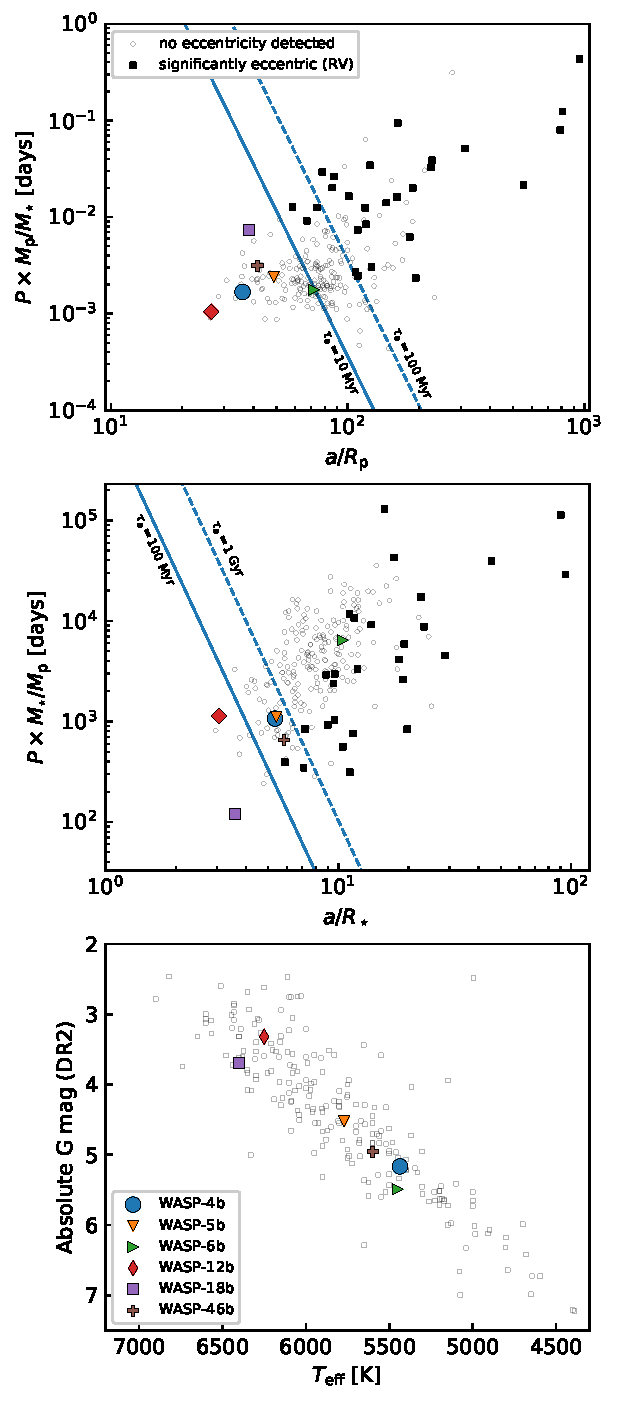
\includegraphics[width=0.48\textwidth]{f5.pdf}
	\end{center}
	\vspace{-0.4cm}
	\caption{
  {\bf Predicted hot Jupiter period changes from linear radial
  velocity trends.} Including WASP-4b, 16 of 51 hot Jupiters from
  \citet{knutson_friends_2014} have shown long-term radial velocity
  trends.  HAT-P-11 is shown, though its signal may be caused
  by stellar activity.  Three hot Jupiters are not shown because
  their radial velocity curves are better described as quadratic
  trends in time: HAT-P-17, WASP-8, and WASP-34.  Objects are ordered
  in the $y$ dimension by the absolute value of d$P$/d$t$.
	\label{fig:pdot_pop}
  \vspace{-0.3cm}
	}
\end{figure}

We identified WASP-4b's decreasing orbital period as part of a search
for tidal orbital decay.  However, most hot Jupiters have companions
outside of $5\,{\rm AU}$ with super-Jovian masses
\citep{knutson_friends_2014,bryan_statistics_2016}.  Line-of-sight
accelerations are correspondingly common in hot Jupiter systems. 

To evaluate the importance of these effects for future transit timing
analyses, we collected the linear radial velocity trends reported by
\citet{knutson_friends_2014}, and computed the expected orbital period
derivatives $\dot{P}_{\rm\,RV} = \dot{v}_{\rm r} P/c$ for each system.
The results are given in Table~4, and visualized for hot Jupiters with
significant ($>$$3\sigma$) linear trends in Figure~\ref{fig:pdot_pop}.

Including WASP-4b, 16 of 51 hot Jupiters surveyed by
\citet{knutson_friends_2014} show a non-zero radial velocity trend.
Therefore around 1 in 3 hot Jupiters is expected to show period
changes commensurate with WASP-4 due to acceleration by outer
companions.  Half of these will be period decreases\footnote{ At a
population level, one would expect half of the line-of-sight
accelerations to be positive, and half negative.  Tidal orbital decay
however is usually negative, and could evenutally manifest as an asymmetry in the
$\dot{P}$ distribution of hot Jupiters.}, and will be an
astrophysical false positive in searches for tidal orbital decay.


\subsection{At what rate is the measurement precision of d$P$/d$t$
increasing?}
\label{sec:fisher}

For hot Jupiters that have been monitored over baselines
exceeding 10 years, secular changes in their orbital periods are
currently being constrained to a precision of $\lesssim$$10~{\rm
msec}\,{\rm yr}^{-1}$ ({\it e.g.}, K.~Patra et al{.} 2020, submitted).
This is roughly commensurate with the level of signal many outer
companions are expected to induce (Figure~\ref{fig:pdot_pop}).

It is therefore pertinent to ask at what point in time further
detections of the light-travel time effect will become routine for hot
Jupiters.  This question is the same as asking: at what rate does the
uncertainty in the quadratic term of Equation~\ref{eq:quadratic_model}
scale with the observing baseline?  We take a Fisher analysis approach
to the problem.  First, we rewrite Equation~\ref{eq:quadratic_model}
as
\begin{align}
  t_{\rm tra} = a_0 + a_1 E + a_2 E^2,
\end{align}
where $a_0\equiv t_0$, $a_1\equiv P$, and $a_2\equiv 0.5\cdot {\rm
d}P/{\rm d}E$.  Following \citet{gould_chi2_2003}, one can show that
if $N$ transit timing measurements are taken uniformly across a
baseline of $\Delta E$ epochs with constant precision $\sigma$, then
the uncertainty of the quadratic term is given by
\begin{align}
  \sigma_{a_2} = 6\sqrt{5}
   \frac{\sigma}{N^{1/2} (\Delta E)^2} \propto (\Delta E)^{-5/2}.
\end{align}
This result implies that a doubled observing baseline yields an
$\approx$5.7-fold improvement in precision on d$P$/d$t$.  If regular
observations continue from ground and space-based observatories,
period derivatives will be measured with precision exceeding
$1~{\rm msec}\,{\rm yr}^{-1}$ within the coming decade.


\section{Conclusions}
\label{sec:conclusions}

From newly acquired radial velocity measurements, we found that WASP-4
is accelerating towards the Earth at $\dot{\gamma} =
-0.0422^{+0.0028}_{-0.0027}\ {\rm m}\,{\rm s}^{-1}\,{\rm day}^{-1}$.
The corresponding light-travel time effect predicts a period decrease
$\dot{\gamma} P/c$ of $-5.94 \pm 0.39~{\rm msec}\,{\rm yr}^{-1}$.  The
majority of the period decrease observed in transits ($\dot{P}= - 8.64
\pm 1.26~{\rm msec}\,{\rm yr}^{-1}$) is therefore explained by the
acceleration of the host star~---~not tidal orbital decay, or apsidal
precession.  The companion causing the acceleration is most likely a
brown dwarf or low-mass star with semi-major axis between
10-100$\,$AU.

Most hot Jupiters have outer companions with masses larger than
Jupiter beyond 5$\,$AU
\citep{knutson_friends_2014,bryan_statistics_2016}. The accelerations
and period changes induced by these outer companions will become an
increasingly large nuisance in the hunt for tidal orbital decay as the
observational baselines get longer.  In particular, the precision with
which the period derivative can be measured from transits scales with
the baseline duration to the power of 5/2 (Section~\ref{sec:fisher}), and
so within a decade many more hot Jupiters should show orbital period
changes due to accelerations from their outer companions.  
To distinguish this effect from tidal decay, further long-term radial
velocity measurements of hot Jupiters are strongly encouraged.

%%%%%%%%%%%%%%%%%%%%%%%%%%%%%%%%%%%%%%%%%%%%%%%%%%%%%%%%%%%%%%%%%%%%%%%%%%%%%%%

% \acknowledgements
% %
% This paper includes data collected by the TESS mission, which are
% publicly available from the Mikulski Archive for Space Telescopes
% (MAST).
% %
% Funding for the TESS mission is provided by NASA's Science Mission
% directorate.
% %
% This work made use of NASA's Astrophysics Data System Bibliographic
% Services.
% %
% Based on observations obtained at the Gemini Observatory, which is
% operated by the Association of Universities for Research in Astronomy,
% Inc., under a cooperative agreement with the NSF on behalf of the
% Gemini partnership: the National Science Foundation (United States),
% National Research Council (Canada), CONICYT (Chile), Ministerio de
% Ciencia, Tecnolog\'{i}a e Innovaci\'{o}n Productiva (Argentina),
% Minist\'{e}rio da Ci\^{e}ncia, Tecnologia e Inova\c{c}\~{a}o (Brazil),
% and Korea Astronomy and Space Science Institute (Republic of Korea).
% %
% Observations in the paper made use of the High-Resolution Imaging
% instrument Zorro at Gemini-South. Zorro was funded by the NASA
% Exoplanet Exploration Program and built at the NASA Ames Research
% Center by Steve B. Howell, Nic Scott, Elliott P. Horch, and Emmett
% Quigley.
% %
% This research has made use of the VizieR catalogue access tool, CDS,
% Strasbourg, France. The original description of the VizieR service was
% published in A\&AS 143, 23.
% %
% This work has made use of data from the European Space Agency (ESA)
% mission {\it Gaia} (\url{https://www.cosmos.esa.int/gaia}), processed
% by the {\it Gaia} Data Processing and Analysis Consortium (DPAC,
% \url{https://www.cosmos.esa.int/web/gaia/dpac/consortium}). Funding
% for the DPAC has been provided by national institutions, in particular
% the institutions participating in the {\it Gaia} Multilateral
% Agreement.
%
% \newline
%

\software{
  \texttt{astrobase} \citep{bhatti_astrobase_2018},
  % \texttt{astroplan} \citep{astroplan2018},
  \texttt{astropy} \citep{astropy_2018},
  \texttt{astroquery} \citep{astroquery_2018},
  % \texttt{BATMAN} \citep{kreidberg_batman_2015},
  \texttt{corner} \citep{corner_2016},
  \texttt{emcee} \citep{foreman-mackey_emcee_2013},
  \texttt{IPython} \citep{perez_2007},
  \texttt{matplotlib} \citep{hunter_matplotlib_2007}, 
	\texttt{MESA} \citep{paxton_modules_2011,paxton_modules_2013,paxton_modules_2015}
  \texttt{numpy} \citep{walt_numpy_2011}, 
  \texttt{pandas} \citep{mckinney-proc-scipy-2010},
  \texttt{radvel} \citep{fulton_radvel_2018},
  % \texttt{scikit-learn} \citep{scikit-learn},
  \texttt{scipy} \citep{jones_scipy_2001}.
}

%
% The following are entries from Table 1 that are not otherwise cited
% in the text
%
\nocite{wilson_wasp-4b_2008}
\nocite{gillon_improved_2009}
\nocite{winn_transit_2009}
\nocite{hoyer_tramos_2013}
\nocite{dragomir_terms_2011}
\nocite{sanchis-ojeda_starspots_2011}
\nocite{nikolov_wasp-4b_2012}
\nocite{ranjan_atmospheric_2014}
\nocite{huitson_gemini_2017}

\bibliographystyle{yahapj}                            
\bibliography{bibliography} 

%% \begin{deluxetable}{} command tell LaTeX how many columns
%% there are and how to align them.
\startlongtable
\begin{deluxetable}{ccccc}
    
%% Keep a portrait orientation

%% Over-ride the default font size
%% Use Default (12pt)
\tabletypesize{\scriptsize}

%% Use \tablewidth{?pt} to over-ride the default table width.
%% If you are unhappy with the default look at the end of the
%% *.log file to see what the default was set at before adjusting
%% this value.

%% This is the title of the table.
\tablecaption{WASP-4b transit times, uncertainties, and references.}
\label{tab:transit_times}

%% This command over-rides LaTeX's natural table count
%% and replaces it with this number.  LaTeX will increment 
%% all other tables after this table based on this number
\tablenum{1}

%% The \tablehead gives provides the column headers.  It
%% is currently set up so that the column labels are on the
%% top line and the units surrounded by ()s are in the 
%% bottom line.  You may add more header information by writing
%% another line between these lines. For each column that requries
%% extra information be sure to include a \colhead{text} command
%% and remember to end any extra lines with \\ and include the 
%% correct number of &s.
\tablehead{
  \colhead{$t_{\rm tra}$ [BJD$_\mathrm{TDB}$]} &
  \colhead{$\sigma_{t_{\rm tra}}$ [days]} &
  \colhead{Epoch} & 
  \colhead{H13?} & 
  \colhead{Reference}
}

%% All data must appear between the \startdata and \enddata commands
% XXX pasted in from selected_transit_times.tex
\startdata
 2454368.59279 &      0.00033 &   -1059 &       1 &           \citet{wilson_wasp-4b_2008} \\
 2454396.69576 &      0.00012 &   -1038 &       1 &          \citet{gillon_improved_2009} \\
 2454697.79817 &      0.00009 &    -813 &       1 &             \citet{winn_transit_2009} \\
 2454701.81280 &      0.00022 &    -810 &       1 &             \citet{hoyer_tramos_2013} \\
 2454701.81303 &      0.00018 &    -810 &       1 &             \citet{hoyer_tramos_2013} \\
 2454705.82715 &      0.00029 &    -807 &       1 &             \citet{hoyer_tramos_2013} \\
 2454728.57767 &      0.00042 &    -790 &       1 &             \citet{hoyer_tramos_2013} \\
 2454732.59197 &      0.00050 &    -787 &       1 &             \citet{hoyer_tramos_2013} \\
 2454740.62125 &      0.00035 &    -781 &       1 &             \citet{hoyer_tramos_2013} \\
 2454748.65111 &      0.00007 &    -775 &       1 &             \citet{winn_transit_2009} \\
 2454752.66576 &      0.00069 &    -772 &       1 &           \citet{dragomir_terms_2011} \\
 2455041.72377 &      0.00018 &    -556 &       1 &             \citet{hoyer_tramos_2013} \\
 2455045.73853 &      0.00008 &    -553 &       1 &  \citet{sanchis-ojeda_starspots_2011} \\
 2455049.75325 &      0.00007 &    -550 &       1 &  \citet{sanchis-ojeda_starspots_2011} \\
 2455053.76774 &      0.00009 &    -547 &       1 &  \citet{sanchis-ojeda_starspots_2011} \\
 2455069.82661 &      0.00029 &    -535 &       1 &          \citet{nikolov_wasp-4b_2012} \\
 2455069.82670 &      0.00028 &    -535 &       1 &          \citet{nikolov_wasp-4b_2012} \\
 2455069.82617 &      0.00038 &    -535 &       1 &          \citet{nikolov_wasp-4b_2012} \\
 2455069.82676 &      0.00031 &    -535 &       1 &          \citet{nikolov_wasp-4b_2012} \\
 2455073.84128 &      0.00026 &    -532 &       1 &          \citet{nikolov_wasp-4b_2012} \\
 2455073.84108 &      0.00029 &    -532 &       1 &          \citet{nikolov_wasp-4b_2012} \\
 2455073.84111 &      0.00023 &    -532 &       1 &          \citet{nikolov_wasp-4b_2012} \\
 2455073.84114 &      0.00018 &    -532 &       1 &          \citet{nikolov_wasp-4b_2012} \\
 2455096.59148 &      0.00022 &    -515 &       1 &             \citet{hoyer_tramos_2013} \\
 2455100.60595 &      0.00012 &    -512 &       1 &  \citet{sanchis-ojeda_starspots_2011} \\
 2455112.64986 &      0.00039 &    -503 &       1 &          \citet{nikolov_wasp-4b_2012} \\
 2455112.65009 &      0.00033 &    -503 &       1 &          \citet{nikolov_wasp-4b_2012} \\
 2455112.65005 &      0.00031 &    -503 &       1 &          \citet{nikolov_wasp-4b_2012} \\
 2455112.65005 &      0.00049 &    -503 &       1 &          \citet{nikolov_wasp-4b_2012} \\
 2455132.72310 &      0.00041 &    -488 &       1 &             \citet{hoyer_tramos_2013} \\
 2455468.61943 &      0.00046 &    -237 &       1 &             \citet{hoyer_tramos_2013} \\
 2455526.16356 &      0.00008 &    -194 &       0 &       \citet{ranjan_atmospheric_2014} \\
 2455828.60375 &      0.00041 &      32 &       1 &             \citet{hoyer_tramos_2013} \\
 2455832.61815 &      0.00041 &      35 &       1 &             \citet{hoyer_tramos_2013} \\
 2455844.66287 &      0.00009 &      44 &       0 &           \citet{huitson_gemini_2017} \\
 2456216.69123 &      0.00006 &     322 &       0 &           \citet{huitson_gemini_2017} \\
 2456576.67556 &      0.00005 &     591 &       0 &           \citet{huitson_gemini_2017} \\
 2456924.61561 &      0.00006 &     851 &       0 &           \citet{huitson_gemini_2017} \\
 2458355.18490 &      0.00024 &    1920 &       0 &                             This work \\
 2458356.52251 &      0.00026 &    1921 &       0 &                             This work \\
 2458357.86101 &      0.00024 &    1922 &       0 &                             This work \\
 2458359.19951 &      0.00025 &    1923 &       0 &                             This work \\
 2458360.53708 &      0.00027 &    1924 &       0 &                             This work \\
 2458361.87539 &      0.00024 &    1925 &       0 &                             This work \\
 2458363.21412 &      0.00027 &    1926 &       0 &                             This work \\
 2458364.55192 &      0.00025 &    1927 &       0 &                             This work \\
 2458365.89064 &      0.00026 &    1928 &       0 &                             This work \\
 2458369.90503 &      0.00027 &    1931 &       0 &                             This work \\
 2458371.24297 &      0.00026 &    1932 &       0 &                             This work \\
 2458372.58136 &      0.00027 &    1933 &       0 &                             This work \\
 2458373.91982 &      0.00027 &    1934 &       0 &                             This work \\
 2458375.25801 &      0.00024 &    1935 &       0 &                             This work \\
 2458376.59621 &      0.00024 &    1936 &       0 &                             This work \\
 2458377.93443 &      0.00026 &    1937 &       0 &                             This work \\
 2458379.27317 &      0.00026 &    1938 &       0 &                             This work \\
 2458380.61097 &      0.00027 &    1939 &       0 &                             This work \\
\enddata

%% Include any \tablenotetext{key}{text}, \tablerefs{ref list},
%% or \tablecomments{text} between the \enddata and 
%% \end{deluxetable} commands

%% General table comment marker
\tablecomments{
    $t_{\rm tra}$ is the measured transit midtime, and $\sigma_{t_{\rm
    tra}}$ is its $1\sigma$ uncertainty.
    $\sigma_{t_0}$ was evaluated from the sampled posteriors by taking
    the maximum of the difference between the 84th percentile
    minus the median, and the median minus the 16th percentile.
    The ``Reference'' column refers to the work describing the
    original observations.
    The ``H13?'' column is 1 if the mid-time value was taken from 
    \citet{hoyer_tramos_2013}.  Otherwise, the mid-time
    came from the column listed in ``Reference''.
    The \citet{hoyer_tramos_2013} BJD$_{\rm TT}$ times are equal to
    BJD$_{\rm TDB}$ for our purposes \citep{urban_explanatory_2012}.
    We omitted the timing measurements from
    \citet{southworth_high-precision_2009}, since there were technical
    problems with the computer clock at the time of
    observation~\citep{nikolov_wasp-4b_2012}.
}
\end{deluxetable}

\vspace{-2cm}
%% \begin{deluxetable}{} command tell LaTeX how many columns
%% there are and how to align them.
\startlongtable
\begin{deluxetable*}{cccccc}
    
%% Keep a portrait orientation

%% Over-ride the default font size
%% Use Default (12pt)
\tabletypesize{\scriptsize}

%% Use \tablewidth{?pt} to over-ride the default table width.
%% If you are unhappy with the default look at the end of the
%% *.log file to see what the default was set at before adjusting
%% this value.

%% This is the title of the table.
\tablecaption{WASP-4b radial velocities.}
\label{tab:rvs}

%% This command over-rides LaTeX's natural table count
%% and replaces it with this number.  LaTeX will increment 
%% all other tables after this table based on this number
\tablenum{2}

%% The \tablehead gives provides the column headers.  It
%% is currently set up so that the column labels are on the
%% top line and the units surrounded by ()s are in the 
%% bottom line.  You may add more header information by writing
%% another line between these lines. For each column that requries
%% extra information be sure to include a \colhead{text} command
%% and remember to end any extra lines with \\ and include the 
%% correct number of &s.
\tablehead{
  \colhead{Time [BJD$_\mathrm{TDB}$]} &
  \colhead{RV [m$\,$s$^{-1}$]} &
  \colhead{$\sigma_{\rm RV}$ [m$\,$s$^{-1}$]} & 
  \colhead{$S$-value} &
  \colhead{Instrument} & 
  \colhead{Provenance}
}

%% All data must appear between the \startdata and \enddata commands
% XXX pasted in from selected_transit_times.tex
\startdata
 2454321.12345 &      42 &   0.42 &       0.42    & HIRES & \citet{knutson_friends_2014} \\
\enddata

%% Include any \tablenotetext{key}{text}, \tablerefs{ref list},
%% or \tablecomments{text} between the \enddata and 
%% \end{deluxetable} commands

%% General table comment marker
\tablecomments{
Table~2 is published in its entirety in a machine-readable format.
The first few entries are shown for guidance regarding form and
content. $S$-values are collected only for the HIRES measurements.
}
\end{deluxetable*}

\vspace{-2cm}
%\renewcommand{\arraystretch}{1.0}

\startlongtable
\begin{deluxetable}{lc}

\tabletypesize{\footnotesize}

\tablenum{4}

%\tablewidth{0pt}

\tablecaption{Best-fit model parameters.}
\label{tab:bestfit}

\tablehead{
  \colhead{Parameter} &
  \colhead{Median Value~(Unc.)\tablenotemark{a}}
}

\startdata
~~~~~~{\it Constant period} &  \\
$t_0$\,[${\rm BJD}_{\rm TBD}$]    & 2455804.515752(+19)(-19)              \\
$P$\,[days]                       & 1.338231466(+23)(-22)                 \\
~~~~~~{\it Constant period derivative} &  \\
$t_0$~[${\rm BJD}_{\rm TBD}$]     & 2455804.515918(+24)(-24)              \\
$P$\,[days]                       & 1.338231679(+31)(-31)                 \\
$dP/dt$                           & $-4.00(+37)(-38) \times 10^{-10}$     \\
~~~~~~{\it Apsidal precession} &  \\
$t_0$~[${\rm BJD}_{\rm TBD}$]     & 2455804.51530(+25)(-31)               \\
$P_{\rm s}$\,[days]               & 1.33823127(+20)(-48)                  \\
$e$                               & $1.92^{+1.93}_{-0.76} \times 10^{-3}$ \\
$\omega_0$\,[rad]                 & 2.40(+38)(-34)                        \\
$d\omega/dE$~[rad\,epoch$^{-1}$]  & $8.70^{+3.01}_{-2.30} \times 10^{-4}$ \\
\enddata
\tablenotetext{a}{
The numbers in parenthesis give the $68\%$ confidence interval for the final
two digits, where appropriate.
}
\end{deluxetable}


\vspace{-2cm}
\startlongtable
\begin{deluxetable*}{lllllllll}
%
\tablecaption{
	Predicted hot Jupiter period changes from linear radial
	velocity trends reported by \citet{knutson_friends_2014}.
\label{tab:pdot_table}
}
%
\tablenum{4}
%
% planet;gammadot;gammadot_pluserr;gammadot_minuserr;comment;pl_name;pl_orbper;Pdot;Pdot_upper_limit;Pdot_lower_limit;Pdot_perr;Pdot_merr;abs_Pdot;K14_significant
\tablehead{
  \colhead{Planet} &
  \colhead{$\dot{\gamma}$ [m$\,$s$^{-1}$$\,$yr$^{-1}$]} &
  \colhead{$+\sigma_{\dot{\gamma}}$ [m$\,$s$^{-1}$yr$^{-1}$]} & 
  \colhead{$-\sigma_{\dot{\gamma}}$ [m$\,$s$^{-1}$yr$^{-1}$]} & 
  \colhead{$P$ [days]} &
  \colhead{$\dot{P}_{\,{\rm RV}}$ [ms$\,$yr$^{-1}$]} &
  \colhead{$+\sigma_{\dot{P}_{\,{\rm RV}}}$ [ms$\,$yr$^{-1}$]} &
  \colhead{$-\sigma_{\dot{P}_{\,{\rm RV}}}$ [ms$\,$yr$^{-1}$]} &
  \colhead{Significant?}
}
%
%FIXME precision
\startdata
HAT-P-2 b & -0.0938 & 0.0067 & 0.0069 & 5.6335158 & -55.62 & 3.97 & 4.09 & 1
\enddata
%
\tablecomments{
  Table~4 is published in its entirety in a machine-readable format.
  A single row is shown here for guidance regarding form and content.
}
%
\end{deluxetable*}



\end{document}
